This chapter serves to summarize the methods and results shown in
this technote. Since the start of data collection, the fine-grained
detector (FGD) in ND280 has provided constraints on the neutrino flux
and neutrino-water interaction modes important to the oscillation
analysis. This technote is an analysis of an independent measurement
of the ND280 constraint using a maximum likelihood estimate in the
Beam and Near Detector Flux Task Force (BANFF) framework with samples
from the pi-zero detector ($\pod$).

Analysis samples have been developed with the $\pod$ to capture a
wide variety of interaction modes in T2K, importantly interactions
classified as charged current quasi-elastic (CCQE) which constitute
the highest cross section in the T2K neutrino energy spectrum. While
the $\pod$ has a larger volume compared to the FGD, which means it
has more neutrino interactions to select, the $\pod$ is less sensitive
to non-CCQE interactions like CC single pion production. This limitation
is largely due to the design of the detector and sample selection
which reduce its $\left(p,\cos\theta\right)$ sensitivity to the lower
energy outgoing muons. The systematic uncertainties inherent in the
samples were controlled for in a similar manner with previous BANFF
analyses.

The $\pod$-only data fit shows very good agreement with the FGD-only
result using the same flux and cross section parameters. Trends in
the postfit parameters like the flux shape and the quantum mechanical
correlation affects on the observable cross section were observed
in both sets of fits. 

Other topics discussed in this chapter are presented in the following
order. First shown is a prediction of the oscillated samples at SK
using the ND constraint in \prettyref{sec:Prediction-of-the}. Possible
analysis improvements are discussed in \prettyref{sec:Analysis-Improvements}.
Finally, the prospect of a joint $\pod$ and FGD fit are discussed
in \prettyref{sec:Future-Prospects:-Joint}.

\section{Prediction of the T2K Oscillation Analysis Samples\label{sec:Prediction-of-the}}

In this section, we analyze the BANFF fit as the input for the oscillation
analysis. We are explicitly NOT performing the oscillation analysis,
but we are building a prediction of the oscillated neutrino samples
using the P-Theta frequentist framework described in the 2017 oscillation
analysis publication\cite{Abe:2017vif}. We then compare the prediction
with the observed neutrino energy spectra of the four CCQE-enriched
samples at Super-Kamiokande (SK). These samples are the FHC mode ($\nu$-mode)
$\numu$ sample, the RHC mode ($\antinu$-mode) $\numubar$ sample,
the $\nu$-mode $\nue$ sample, and the $\antinu$-mode $\nuebar$
sample.

The SK prediction is built with the following ingredients: the flux
and cross section parameter estimates from the BANFF fit parameter
estimates and covariance matrix, the nominal set of SK detector systematics
in the frequentist analysis software, and the full three-flavor oscillation
probabilities. The full three-flavor oscillation parameters used are
the same as listed in TABLE II in the 2018 CP violation search paper\cite{Abe:2018wpn},
which are shown in \prettyref{tab:Oscillation-parameters-used} for
convenience. The observed spectra are also taken from the 2018 CP
violation search paper, which had a integrated luminosity of $2.2\times10^{21}$
POT.

The spectra are shown in the following order. First are the of the
$\numu$ CCQE and $\numubar$ CCQE-enriched samples together shown
in \prettyref{fig:Predicted-reconstructed-neutrino}. Next is the
$\nue$ CCQE-enriched sample shown in \prettyref{fig:Reconstructed-nue-CCQE-enriched}.
Finally is the $\nuebar$ CCQE-enriched sample shown in \prettyref{fig:Reconstructed-nuebar-CCQE-enriched}.
The integrated spectra are tabulated in \prettyref{tab:Number-of-events-SK-CCQE}.

\begin{table}
\caption[Oscillation Parameters Used as Inputs for Studies of Simulated Data]{Oscillation parameters used as inputs for studies of simulated data.\label{tab:Oscillation-parameters-used}}

\centering{}%
\begin{tabular}{lcc}
\toprule 
Parameter & Value & Units\tabularnewline
\midrule
\midrule 
Mass hierarchy & \multicolumn{2}{c}{Normal}\tabularnewline
$\Delta m_{21}^{2}$ & 7.53 & $10^{-5}\text{ eV}^{2}/c^{4}$\tabularnewline
$\left|\Delta m_{32}^{2}\right|$ & 2.509 & $10^{-3}\text{ eV}^{2}/c^{4}$\tabularnewline
$\sin^{2}\theta_{23}$ & 0.528 & 1\tabularnewline
$\sin^{2}2\theta_{12}$ & 0.846 & 1\tabularnewline
$\sin^{2}2\theta_{13}$ & 0.0857 & 1\tabularnewline
$\deltacp$ & -1.601 & rad\tabularnewline
$e^{-}$ density & 2.6 & $\text{g}/\text{cm}^{3}$\tabularnewline
Baseline length & 295 & km\tabularnewline
$\nu$-mode luminosity & 14.7 & $10^{20}$ POT\tabularnewline
$\antinu$-mode luminosity & 7.6 & $10^{20}$ POT\tabularnewline
\bottomrule
\end{tabular}
\end{table}

\begin{figure}
\begin{centering}
\subfloat[Prediction]{\begin{centering}
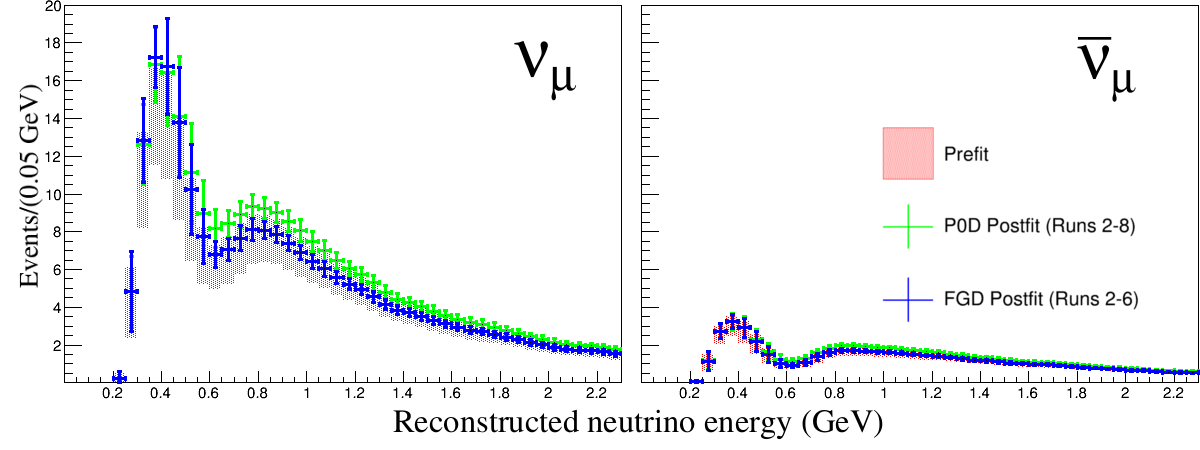
\includegraphics[width=0.8\textwidth]{Chapters/Figures/Discussion/hNumuNumubarPrediction}
\par\end{centering}
}
\par\end{centering}
\begin{centering}
\subfloat[Observed]{\begin{centering}
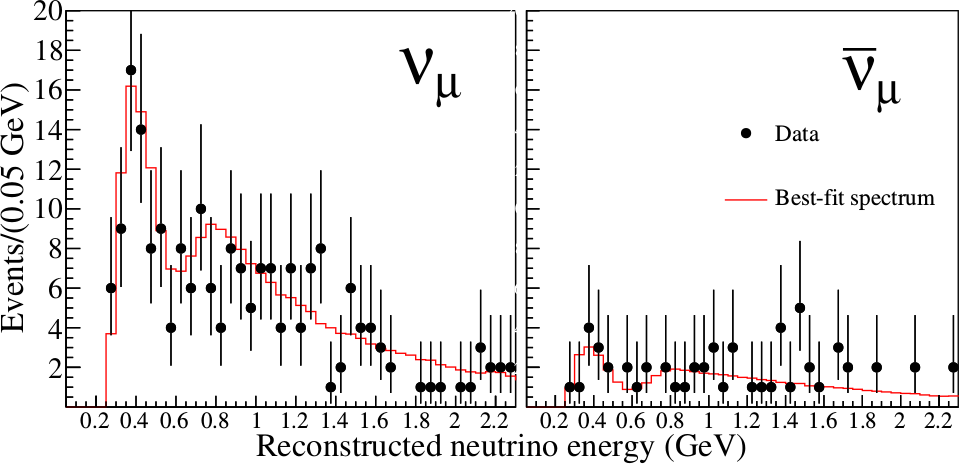
\includegraphics[width=0.8\textwidth]{Chapters/Figures/Discussion/numu_numubar_PRL1211718022018}
\par\end{centering}
}
\par\end{centering}
\caption[Reconstructed $\numu$ and $\numubar$ CCQE-enriched Energy Distributions
at SK]{Reconstructed $\protect\numu$ (left) and $\protect\numubar$ (right)
CCQE-enriched energy distributions at SK. The top figure is the predicted
spectra while the bottom is the observed spectra. The observed spectra
is taken from the 2018 CP violation search publication\cite{Abe:2018wpn}.
\label{fig:Predicted-reconstructed-neutrino}}
\end{figure}

\begin{figure}
\begin{centering}
\subfloat[Prediction]{\begin{centering}
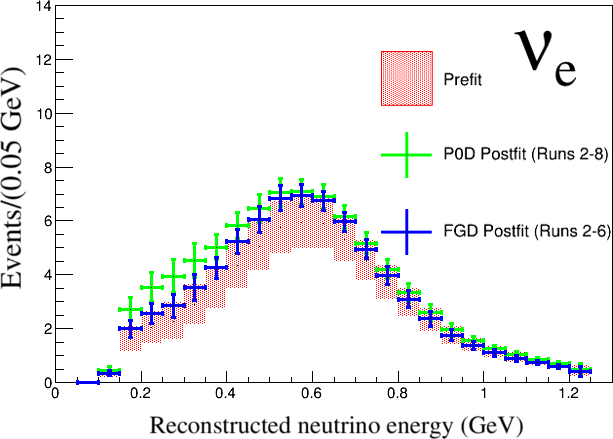
\includegraphics[height=1.9in]{Chapters/Figures/Discussion/hNueFHCPrediction}
\par\end{centering}

}\subfloat[Observed]{\begin{centering}
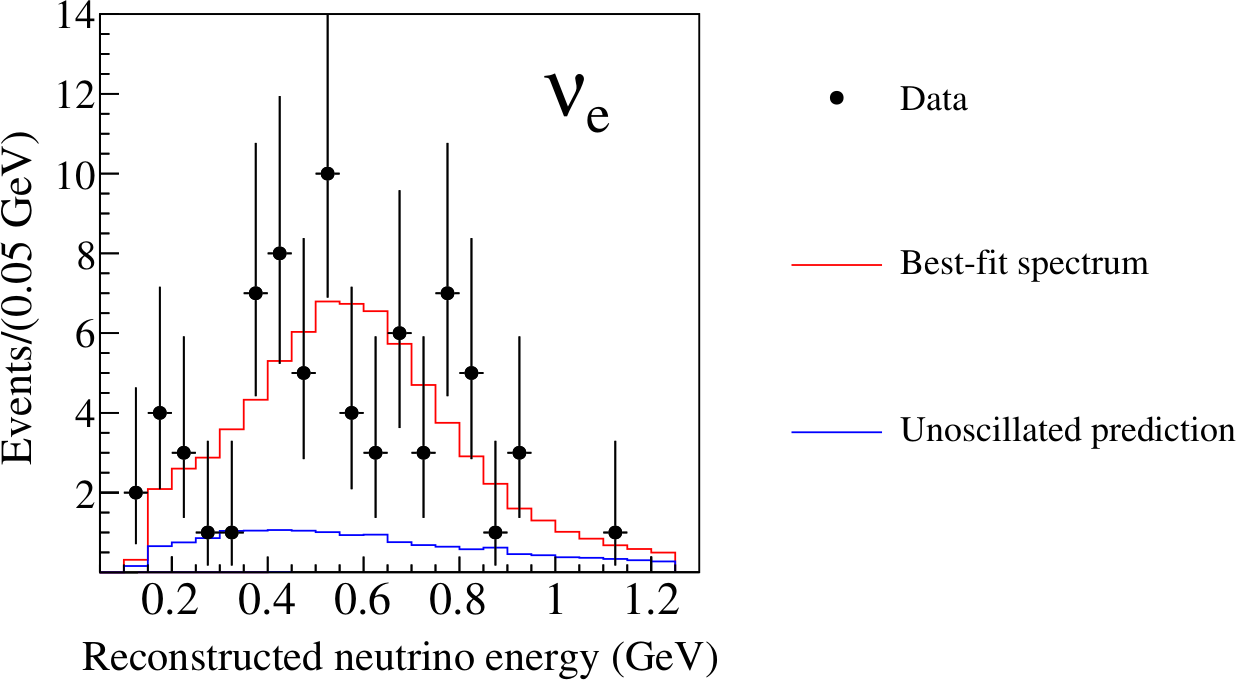
\includegraphics[height=1.9in]{Chapters/Figures/Discussion/nue_PRL1211718022018}
\par\end{centering}
}
\par\end{centering}
\caption[Reconstructed $\nue$ CCQE-enriched Energy Distribution at SK]{Reconstructed $\protect\nue$ CCQE-enriched energy distribution at
SK. The observed spectra is taken from the 2018 CP violation search
publication\cite{Abe:2018wpn}.\label{fig:Reconstructed-nue-CCQE-enriched}}

\end{figure}

\begin{figure}
\begin{centering}
\subfloat[Prediction]{\begin{centering}
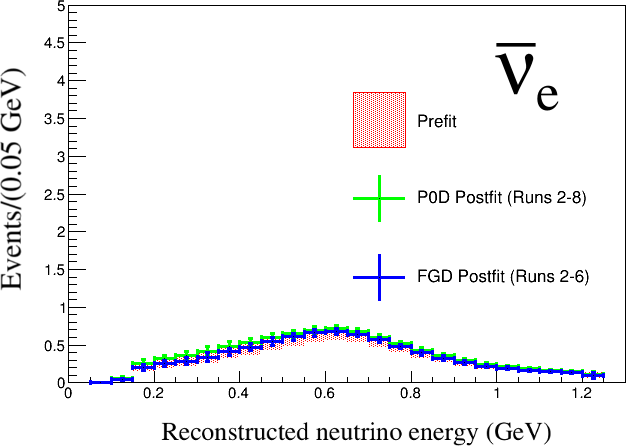
\includegraphics[height=1.9in]{Chapters/Figures/Discussion/hNuebarRHCPrediction}
\par\end{centering}
}\subfloat[Observed]{\begin{centering}
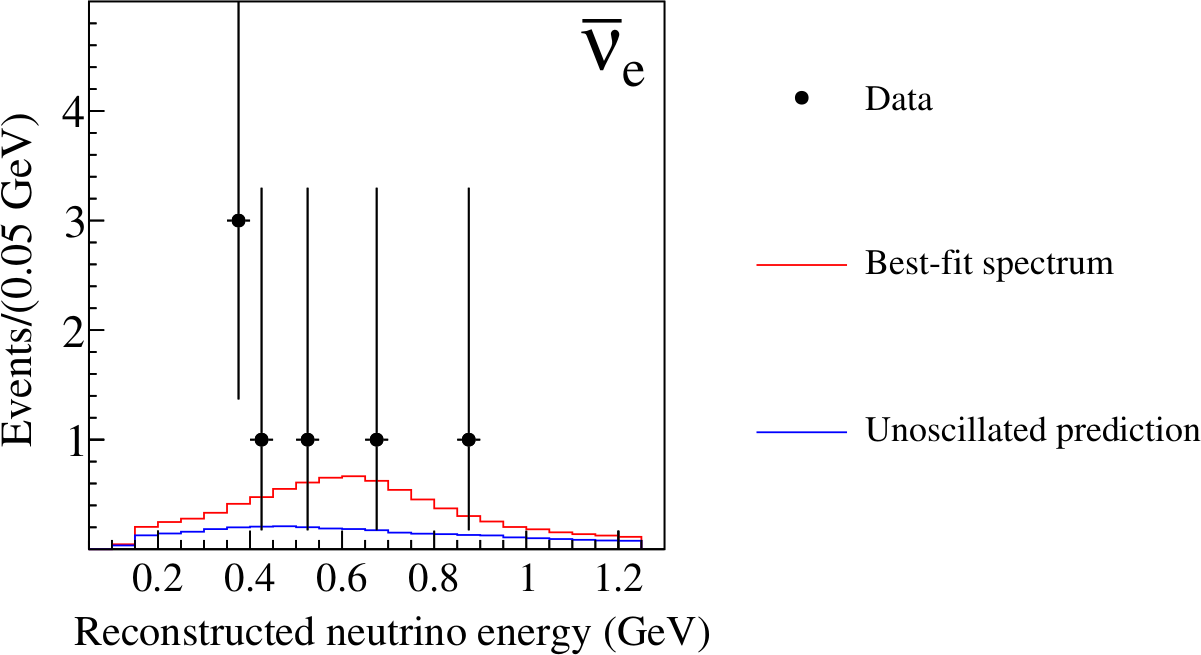
\includegraphics[height=1.9in]{Chapters/Figures/Discussion/nuebar_PRL1211718022018}
\par\end{centering}
}
\par\end{centering}
\caption[Reconstructed $\nue$ CCQE-Enriched Energy Distribution at SK]{Reconstructed $\protect\nuebar$ CCQE-enriched energy distribution
at SK. The observed spectra is taken from the 2018 CP violation search
publication\cite{Abe:2018wpn}.\label{fig:Reconstructed-nuebar-CCQE-enriched}}
\end{figure}

\begin{table}
\caption[Number of Events Expected in the SK CCQE-enriched Samples]{Number of events expected in the SK CCQE-enriched samples.\label{tab:Number-of-events-SK-CCQE}}

\centering{}%
\begin{tabular}{ccccc}
\toprule 
 & Prefit & $\pod$-only & FGD-only & Observed\tabularnewline
\midrule
\midrule 
$\numu$ CCQE ($<2.3$ GeV) & 207.34 & 252.41 & 228.07 & 201\tabularnewline
$\numubar$ CCQE ($<2.3$ GeV) & 49.67 & 58.14 & 52.47 & 57\tabularnewline
$\nue$ CCQE ($<1.3$ GeV) & 65.61 & 83.01 & 74.71 & 74\tabularnewline
$\nuebar$ CCQE ($<1.3$ GeV) & 7.74 & 9.03 & 8.15 & 7\tabularnewline
\bottomrule
\end{tabular}
\end{table}

We observe that each $\pod$-only predicted spectrum is systematically
higher than each FGD-only predicted spectrum. However, the more interesting
differences are the integrated prediction. While the FGD-only prediction
has better agreement with both the $\nue$ and $\numu$ CCQE samples,
the $\pod$-only prediction is agrees well with the $\numubar$ CCQE
sample. It is difficult to judge the agreement of the $\nuebar$ CCQE
sample due to small statistics. However, this all suggests that including
the $\pod$ data samples can improve the ND constraint in RHC mode.

\section{Analysis Improvements\label{sec:Analysis-Improvements}}

Looking forward, the $\pod$-only analysis can be improved significantly.
The $\pod$ selections in this technote are simplistic compared to
the recent developments in the T2K experiment. The author was a part
of the second generation cross section analysis of single pion production
in the $\pod$, which utilized deep learning techniques, to select
a relatively pure CC-$1\pi$ sample. These details are provided in
Appendix \prettyref{app:podcc1pi}. Additionally, the $\pod$ $\numubar$
CC-$0\pi$ analysis\cite{Campbell2018a} was able to achieve a high-purity
CCQE-like sample using almost identical cuts as presented in this
technote. However, both the CC-$1\pi$ and CC-$0\pi$ analyses use
cuts that are not yet available in the BANFF framework due to technical
difficulties and lack of expertise in the collaboration.

Also more validation studies could be done to understand the sensitivity
of the $\pod$ samples. A test of the biases of the fit parameters
requires fitting an ensemble of ``fake data'' sets, which are variations
of the Asimov set. This all requires significant amount of computational
time to complete\footnote{Also not to mention the carbon footprint left afterwards.}.

There are other possible improvements to the ND constraint analysis
using the methods developed for machine learning applications. The
following two sections are on topics to improve the BANFF fit analysis
in its current state. These methods are quite general and rely on
the fundamentals of parameter estimation techniques in statistics.
A section summary is provided to summarize their details.

First is a discussion on applying a different regularization strength.
Second is a method to reduce the number of effective bin normalization
parameters using a different penalty function called the Lasso.

\subsection{Regularization Strength}

Recall that the BANFF ND constraint test statistic is defined as

\[
\begin{aligned}\chi_{\text{ND280}}^{2} & =\chi_{\text{LLR}}^{2}\left(\vec{N}^{d},\vec{N}^{p}\right)+\chi_{\text{Penalty}}^{2}\left(\Delta\vec{y}\right)\end{aligned}
\]
where $\vec{N}^{d}$ and $\vec{N}^{p}$ are the binned data and prediction
measurements, respectively, and $\Delta\vec{y}$ is the difference
between postfit and prefit parameter values in the fit. This equation
is similar to the general class of parameter regression using regularization
\cite{springer_series978-0-387-84858-7} 
\begin{equation}
\begin{aligned}\hat{\beta} & =\underset{f\in\mathcal{F},\beta\in\mathbb{R}^{d}}{\text{argmin}}\left\{ L\left(\eta,f\left(\vec{\beta}\right)\right)+\lambda J\left(f\right)\right\} \end{aligned}
,\label{eq:GeneralRegularization}
\end{equation}
where $L$ is a loss function\footnote{$L$ is also called an objective function.}
of measurements $\eta$, $J\left(f\right)$ is a penalty function,
$f\left(\vec{\beta}\right)$ is a $d$-dimensional function of $\vec{\beta}$,
$\lambda$ is the regularization parameter, and $\mathcal{F}$ is
a space of function on which $J\left(f\right)$ is defined. In regularized
regression problems, the penalty term serves to solve an ill posed
problem by adding external information. Similarly, the regularization
parameter controls the importance of the penalty. We recognize that
the loss function $L$ is the log-likelihood ratio term $\chi_{\text{LLR}}^{2}$,
and penalty term is $J=\chi_{\text{Penalty}}^{2}$ with regularization
strength $\lambda=1$.

In defining the BANFF test statistic in \prettyref{chap:BANFF-Likelihood},
the regularization term $\lambda$ was set to 1 without justification.
We can test the effectiveness of this choice using cross-validation.
Cross-Validation provides an estimate on the prediction error as well
as determines the ``optimal'' choice of regularization. In cross-validation,
the input data is randomly split into $K$ equal sized partitions.
For the $k\in K$ data partition, we fit the model to the other $K-1$
parts of the data and calculate a prediction error $P$.

In this verification of the regularization strength, the test statistic
is altered to include a regularization term

\begin{equation}
\begin{aligned}\chi_{\text{ND280}}^{2} & =\chi_{\text{LLR}}^{2}+\lambda\chi_{\text{Penalty}}^{2}\left(\vec{y}\right)\\
 & =\chi_{\text{LLR}}^{2}+\lambda\left(\vec{y}-\vec{y}_{0}\right)^{T}V^{-1}\left(\vec{y}-\vec{y}_{0}\right),
\end{aligned}
\label{eq:RegularizedDeltaChi2ND280}
\end{equation}
and the data is split into $K=5$ partitions. The prediction error,
$P$, in this analysis is defined as 
\begin{equation}
P_{k}\left(\left(\chi_{\text{train}}^{2}\right)^{-k},\left(\chi_{\text{test}}^{2}\right)^{k}\right)=\left|\left(\chi_{\text{train}}^{2}\right)^{-k}-\left(\chi_{\text{test}}^{2}\right)^{k}\right|\label{eq:predictionerror}
\end{equation}
where $\left(\chi_{\text{train}}^{2}\right)^{-k}$ is the fitted model
statistic on all but the $k$th partition, and $\left(\chi_{\text{test}}^{2}\right)^{k}$
is prediction from the fitted model on the $k$th partition. This
definition of $P$ is useful since the penalty terms cancel, leaving
only the difference in log-likelihood terms. The optimal regularization
strength is determined by minimizing the cross-validation error, 
\begin{equation}
\begin{aligned}\text{CV}\left(\lambda\right) & =\left\langle \left|\chi_{\text{train}}^{2}-\chi_{\text{test}}^{2}\right|\right\rangle \\
 & =\frac{1}{5}\sum_{k=1}^{5}P_{k}\left(\left(\chi_{\text{train}}^{2}\right)^{-k},\left(\chi_{\text{test}}^{2}\right)^{k}\right),
\end{aligned}
\label{eq:CVerror}
\end{equation}
which is the average prediction error.

Results of the cross-validation are shown in \prettyref{fig:Cross-validation}.
We see that while the penalty strength of $\lambda=1$ nearly minimizes
the cross-validation error, slightly larger penalties are preferred.
The cross-validation error curve is minimized roughly at $\lambda=1.4$,
and it is roughly quadratic in the neighborhood around the minimum.
Therefore, a more regularized solution is preferred with the data
sample.

\begin{figure}
\begin{centering}
\subfloat[Wide view]{\begin{centering}
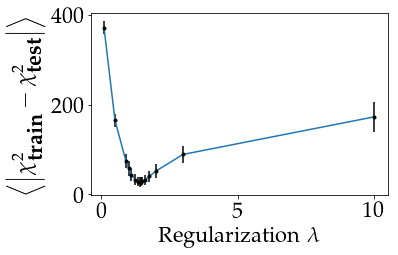
\includegraphics[width=0.45\textwidth]{Chapters/Figures/Discussion/CrossValidationScan}
\par\end{centering}

}\subfloat[Narrow view]{\begin{centering}
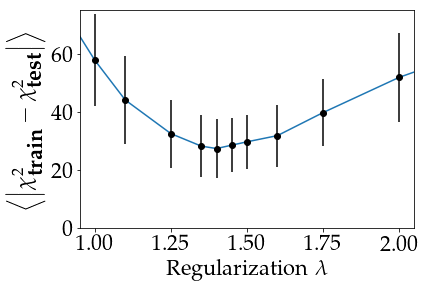
\includegraphics[width=0.45\textwidth]{Chapters/Figures/Discussion/CrossValidationScanZoom}
\par\end{centering}
}
\par\end{centering}
\caption[Cross-Validation Curve for the BANFF Fit Regularization Strength.]{Cross-validation curve for the BANFF fit regularization strength.
Figure (a) examines the cross-validation error for a wide range of
regularization strengths. Figure (b) zooms in on the minimized error.
The error bars shown are statistical only.  \label{fig:Cross-validation}}

\end{figure}

Another data fit with $\lambda=1.4$ was performed with the following
results. The MINUIT optimization routine required 175602 (149661)
iterations to find the global minimum at $\hat{\chi}_{\text{ND}280}^{2}=1344.89$
($1412.28$) with the regularized (non-regularized) penalty term.
The flux parameters have significantly reduced uncertainties compared
to the $\lambda=1$ result. The cross section parameters are relatively
the same as before except for the CC coherent uncertainties which
are much smaller. The was no observed changes in the bin normalization
parameters as well. This suggests that the flux covariance matrix
input needs to reexamined for future BANFF fit analyses. The postfit
parameters are presented in Appendix \prettyref{app:Regularized-Solution}.

\subsection{Alternative Penalty}

Consider solving the linear regression problem 
\begin{equation}
\vec{\eta}=X\vec{\beta}\label{eq:LinearProblem}
\end{equation}
where $X$ is a $p\times d$ matrix of $d$ model features from $p$
measurements, $\vec{\beta}$ is a vector of regression weights with
$p$ rows, and $\vec{\eta}$ is a response vector. There are many
approaches to solving \eqref{eq:LinearProblem} using \eqref{eq:GeneralRegularization}.
A popular solution is the $l_{2}$-regularization constraint\cite{springer_series978-0-387-84858-7}

\begin{equation}
\underset{\vec{\beta}\in\mathbb{R}^{d}}{\text{argmin}}\left\{ L\left(\vec{\eta},\vec{\beta}\right)+\lambda\sum_{i}\left|\beta_{i}\right|^{2}\right\} \label{eq:RidgeRegressionGeneral}
\end{equation}
where the sum of squares of the weights $\beta_{i}$ sets the constraint
and $L$ is the loss function. A popular choice of $L$ is using ordinary
least squares 
\[
L\left(\vec{\eta},\vec{\beta}\right)=\sum_{j}\left|\vec{\eta}-X\vec{\beta}\right|^{2},
\]
which provides the lowest variance in parameter weights. 

With some algebra, we can rewrite the BANFF test statistic \eqref{eq:minBANFFDeltaChiSqr}
into the form of \eqref{eq:RidgeRegressionGeneral}. We again recognize
$\chi_{\text{LLR}}^{2}$ is the loss function $L$ which leaves the
penalty term to be tackled. The (inverse) covariance matrix is symmetric
and real and can be decomposed as
\[
V^{-1}=U^{T}\Lambda U
\]
where $U$ and $\Lambda$ are the matrix of the eigenvectors and eigenvalues,
respectively, of $V^{-1}$. Since the eigenvalues are real and positive,
the matrix $\Lambda$ can be expressed as the square of a diagonal
matrix $\Gamma$
\[
\Lambda=\Gamma^{2}.
\]
We can now rewrite the penalty term as an inner product of two vectors.
\[
\begin{aligned}\chi_{\text{Penalty}}^{2} & =\left(\Delta\vec{y}\right)^{T}V^{-1}\left(\Delta\vec{y}\right)\\
 & \left(\Delta\vec{y}\right)^{T}U^{T}\Gamma^{2}U\left(\Delta\vec{y}\right)\\
 & =\left(\Gamma U\Delta\vec{y}\right)^{T}\left(\Gamma U\Delta\vec{y}\right).
\end{aligned}
\]
If we let $\vec{\psi}=\Gamma U\Delta\vec{y}$, then the penalty term
becomes
\[
\begin{aligned}\chi_{\text{Penalty}}^{2} & =\left(\vec{\psi}\right)^{T}\vec{\psi}=\sum_{j}\left|\psi_{j}\right|^{2}\end{aligned}
\]
and test statistic is now
\begin{equation}
\begin{aligned}\chi_{\text{ND280}}^{2} & =\chi_{\text{LLR}}^{2}\left(N^{d},N^{p}\right)+\left|\left|\psi\right|\right|_{2}^{2}\end{aligned}
,\label{eq:DeltaChiSqND280RidgeRegressionForm}
\end{equation}
where $\left|\left|\ \right|\right|_{2}^{2}$ is shorthand for the
$l_{2}$-regularization constraint sum of squares. We see that the
BANFF test statistic is indeed a $l_{2}$-regularized solution with
$\Delta\vec{y}$, recast as $\vec{\psi}$, acting as the parameter
weight vector and has the regularization strength $\lambda=1$.

Consider now another solution to \eqref{eq:LinearProblem} using the
$l_{1}$-regularization constraint or least absolute shrinkage and
selection operator (Lasso)\footnote{The Lasso or $l_{1}$-regularization constraint is commonly employed
in parameter estimation problems in linear systems. The Lasso has
been shown to work with generalized linear models\cite{JSSv033i01}.}

\begin{equation}
\underset{\vec{\beta}\in\mathbb{R}^{d}}{\text{argmin}}\left\{ L\left(\vec{\eta},\vec{\beta}\right)+\lambda\left|\left|\beta\right|\right|_{1}\right\} ,\label{eq:LassoRegressionGeneral}
\end{equation}
where $\left|\left|\ \right|\right|_{1}$ indicates the sum of absolute
values of the parameter weight terms. What is unique about the Lasso
is its ability to promote model solutions with few nonzero coefficient
weights, sometimes called sparse solutions. In other words, predictor
parameters with no model impact are excluded in the solution using
the $l_{1}$-regularized constraint. Thus the Lasso has the advantage
of providing an interpretable model in situations with very high parameter
spaces. However, the Lasso does not handle highly correlated variables
very well. This is overcome by combining the Lasso with $l_{2}$-regularization
which is called the elastic net constraint
\[
\underset{\vec{\beta}\in\mathbb{R}^{d}}{\text{argmin}}\left\{ L\left(\vec{\eta},\vec{\beta}\right)+\lambda\left(\frac{1}{2}\left(1-\alpha\right)\left|\left|\beta_{i}\right|\right|_{2}^{2}+\alpha\left|\left|\beta_{i}\right|\right|_{1}\right)\right\} ,
\]
where $\alpha$ is the ``budget'' between the Lasso and $l_{2}$-regularization.
The results of using the Lasso and elastic net with highly correlated
variables is shown in \prettyref{fig:The-Lasso-vs-elastic-net}. The
elastic net controls for strong within-group correlations and has
a unique solution. Further details about the Lasso and elastic net
can be found in the following reference \cite{alma991031702535903361}.

\begin{figure}
\begin{centering}
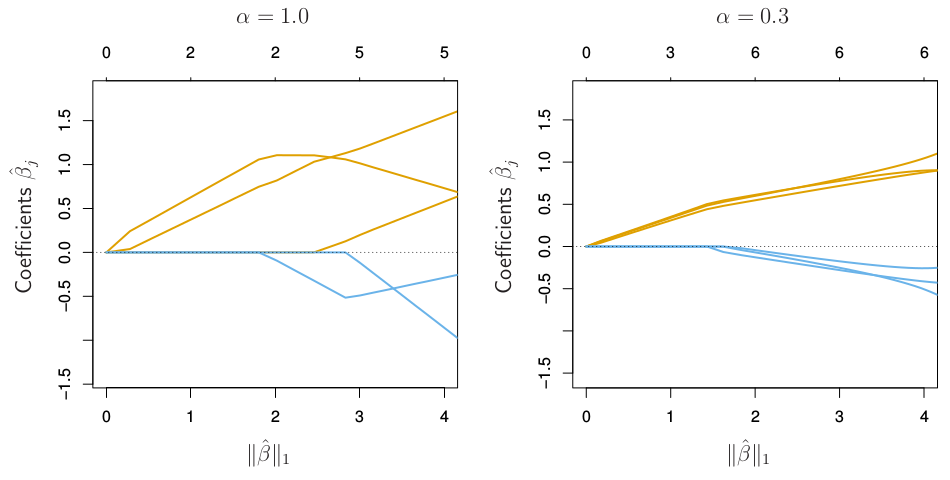
\includegraphics[width=0.75\textwidth]{Chapters/Figures/Discussion/LassoVsElasticNet}
\par\end{centering}
\caption[The Lasso vs Elastic Net Constraint]{The Lasso vs elastic net constraint. Six variables are shown and the
highly correlated variables are in groups of three. The Lasso estimate,
left, estimate exhibits erratic behavior as the regularization strength
$\lambda$ is varied. The elastic net, right, pulls highly correlated
variables together. In both panels, the vertical axis is the magnitude
of the parameter weights (coefficients), the bottom horizontal axis
is the regularization strength as measured by the estimate$\left|\left|\hat{\beta}\right|\right|_{1}$,
and top horizontal axis is the count of non-zero parameter weights.
This figure was taken directly from the following reference\cite{alma991031702535903361}.
\label{fig:The-Lasso-vs-elastic-net}}

\end{figure}

We can potentially reduce the dimensionality of the ND constraint
by utilizing the elastic net. Using the elastic net constraint provides
a data-driven method to determine the number of important bin normalizations
in the analysis. The method to define the fit binning described in
\prettyref{chap:P0DinBANFF} would be unchanged. What changes is that
instead of merging fit bins prior to the fit, the elastic net determines
which bin normalizations are important or not important. Along with
cross-validation, fit bins with minimal to no impact on the fit can
be excluded or combined with important fit bins. Then the best fit
parameters and covariance matrix using the current BANFF machinery
can still be found.

Another possibility in the future is for the BANFF fit to use the
elastic net to directly estimate the flux and cross section parameters.
The challenge with this approach is that using non-Gaussian priors,
the covariance matrix is no longer calculable using the Hess matrix.
This is a general critique of the BANFF fit postfit error estimates
since there are non-Gaussian priors for many of the cross section
parameters. Instead, bootstrap methods could be employed to infer
the parameter covariances. This is further discussed in the following
reference \cite{springer_series978-0-387-84858-7}.

\subsection{Analysis Improvement Summary}

We have explored topics that can potentially improve the BANFF fit
analysis. Improved sensitivity to CC-$0\pi$ and CC-$1\pi$ model
parameters using already developed $\pod$ selections is possible
if the BANFF software is updated. We also examined two topics developed
in machine learning practices to improve parameter estimation. The
first was a study on the strength of the penalty term. It was shown
that we can find a tuning, or regularization, parameter for the penalty
term that reduces the parameter variance but at cost of some parameter
bias. The second topic was a general discussion on using a different
BANFF fit test statistic called the Lasso. The Lasso has the attractive
feature, without user input, of determining which parameters are unimportant
in a model fit. The implication here is that the number bin normalization
parameters in the BANFF fit can be effectively shrunk using the data
itself.

\section{Future Prospects: Joint \podtitle{}+FGD Fit\label{sec:Future-Prospects:-Joint}}

There are potential improvements in a ``joint'' $\pod$+FGD BANFF
fit for the T2K experiment. As shown in the previous chapter, the
number of neutrino-carbon and neutrino-oxygen events can be significantly
increased by including the $\pod$ data. This will enhance the fit's
sensitivity, and possibly improve constraints on poorly constrained
parameters like that of the 2p2h interaction. There is an additional
observed tension in each of the predicted SK sample spectrum between
the $\pod$-only and FGD-only fits, which needs to be resolved.

However, since the fits were performed on different T2K run periods,
an equal POT exposure comparison is useful here. Proposing to run
a ``joint'' $\pod$+FGD ND constraint using T2K runs 2 - 8, the
updated neutrino-nucleus exposures are given in \prettyref{tab:Neutrino-exposure-P0DFGD-EqualPOT}.
We see that while the number of neutrino-carbon events is still larger
in the $\pod$. However, the $\pod$ has 25\% fewer neutrino-oxygen
events in FHC mode and 9\% more in RHC mode. We can estimate the fractional
statistical error ($\delta N$) reduction in a joint fit using the
data from \prettyref{tab:Neutrino-exposure-P0DFGD-EqualPOT} assuming
the FGD fit is the nominal ND constraint. The fractional errors decrease
approximately by
\[
\begin{aligned}\delta N_{^{12}C}^{\text{FGD1-FHC}} & =\frac{1}{\sqrt{N_{^{12}C}^{\text{FGD1-FHC}}}}\overset{+\pod\text{ Air}}{\longrightarrow}\frac{1}{\sqrt{(1+2.01)N_{^{12}C}^{\text{FGD1-FHC}}}}\sim\frac{1}{\sqrt{3.01}}\approx0.576\\
\delta N_{^{16}O}^{\text{FGD2-FHC}} & =\frac{1}{\sqrt{N_{^{16}O}^{\text{FGD2-FHC}}}}\overset{+\pod\text{ Water}}{\longrightarrow}\frac{1}{\sqrt{(1+0.72)N_{^{12}C}^{\text{FGD1-FHC}}}}\sim\frac{1}{\sqrt{1.72}}\approx0.762\\
\delta N_{^{12}C}^{\text{FGD1-RHC}} & =\frac{1}{\sqrt{N_{^{12}C}^{\text{FGD1-RHC}}}}\overset{+\pod\text{ Air}}{\longrightarrow}\frac{1}{\sqrt{(1+1.60)N_{^{12}C}^{\text{FGD1-RHC}}}}\sim\frac{1}{\sqrt{2.60}}\approx0.620\\
\delta N_{^{16}O}^{\text{FGD2-RHC}} & =\frac{1}{\sqrt{N_{^{16}O}^{\text{FGD2-RHC}}}}\overset{+\pod\text{ Water}}{\longrightarrow}\frac{1}{\sqrt{(1+1.04)N_{^{12}C}^{\text{FGD2-RHC}}}}\sim\frac{1}{\sqrt{2.04}}\approx0.700,
\end{aligned}
\]
where combinations of FGD1/2 and FHC/RHC represent the FGD in the
different beam modes, and an right-pointing arrow indicates adding
the $\pod$ data. These results indicate a fractional statistical
error reductions around $1/\sqrt{2}$ for both neutrino-oxygen events
and also potentially stronger flux constraint from higher statistics.

Employing both the FGD and $\pod$ in a joint BANFF fit was attempted,
but the fit failed to converge due to machine precision limits. Including
both detectors with the FGD parameterization described in reference
\cite{Bienstock2017} more than doubles the number of parameters and
events than a single detector-only fit. This not only requires more
iterations to ensure the test statistic global minimum is found, but
also requires more calculations per iteration as well. For instance,
the required time to ensure the joint $\pod$+FGD Asimov fit started
at the global minimum took 10 times larger than the $\pod$-only Asimov
fit. So parameter shrinkage must be performed on both analyses if
reasonable computational speed and maximum statistical power are desired
in the BANFF fit. This is further discussed in Appendix \prettyref{chap:Computing-Resources}.

\begin{landscape}%

\begin{table}
\caption[Neutrino-Nucleon Exposure on Target Elements in a $\pod$+FGD Joint
Fit]{Neutrino-nucleon exposure on target elements in a joint $\pod$ and
FGD analysis using T2K runs 2 - 8.\label{tab:Neutrino-exposure-P0DFGD-EqualPOT}}

\centering{}%
\begin{tabular}{ccccccc}
\toprule 
\multirow{2}{*}{Detector} & \multicolumn{2}{c}{POT $\left(10^{20}\right)$} & kg POT & \multicolumn{3}{c}{$\pod$-to-FGD (kg POT)}\tabularnewline
 & FHC & RHC & $\left(10^{24}\right)$ & \ce{^{12}C} & \ce{^{16}O} & other\tabularnewline
\midrule
\midrule 
$\pod$ Water-out & 7.872 & - & 2.81 & \multirow{2}{*}{2.01} & \multirow{2}{*}{-} & \multirow{2}{*}{4.64}\tabularnewline
FGD1 & 11.529 & - & 1.14 &  &  & \tabularnewline
\midrule 
$\pod$ Water-In & 3.657 & - & 2.00 & \multirow{2}{*}{5.36} & \multirow{2}{*}{0.724} & \multirow{2}{*}{4.06}\tabularnewline
FGD2 & 11.529 & - & 1.12 &  &  & \tabularnewline
\midrule 
$\pod$ Water-out & - & 3.382 & 1.207 & \multirow{2}{*}{1.60} & \multirow{2}{*}{-} & \multirow{2}{*}{3.69}\tabularnewline
FGD1 & - & 6.234 & 0.614 &  &  & \tabularnewline
\midrule 
$\pod$ Water-In & - & 2.852 & 1.56 & \multirow{2}{*}{7.72} & \multirow{2}{*}{1.04} & \multirow{2}{*}{5.85}\tabularnewline
FGD2 & - & 6.234 & 0.606 &  &  & \tabularnewline
\bottomrule
\end{tabular}
\end{table}

\end{landscape}%
